\documentclass[10pt]{article}
\usepackage[utf8]{inputenc}
\usepackage[margin=0.5in]{geometry}
\usepackage{graphicx}
\usepackage{wrapfig}


\begin{document}

{\LARGE AutoGeocoding Update}


This document briefly summarizes the findings from our initial assessment of the autogeocoding activity.  Data limitations significantly hindered our capacity to conduct these comparisons, and thus limit the conclusions of this report\footnote{These results are built upon a subset of all documents used to geocode Malawi, contrasted to the final produced Malawi dataset.  As such, it was impossible for any geocoder to attain perfect accuracy, and it is unknown what the delta is between achievable accuracy and perfect accuracy.  These results can only be interpreted as (a) a worst-case example for geocoding, and (b) a relative assessment of the capacity of various geocoders.  They should not be interpreted as an estimate of the absolute accuracy of any particular geocoder.}.  Noting these limitations, we draw three conclusions and make two recommendations.

\begin{enumerate}
\item \textbf{Data Providence and Chains} - previous human geocoding efforts did not provide enough information to link project documents to individual geocoded locations. This was due to a lack of specificity in the linkages ('See Google Drive'), a failure to save the information used to generate geocodes, and a lack of clear standards for geocoders.  Further, there is no consistent record of inter- (or intra-) coder reliability amongst our human coders. This severly hampers efforts to determine the relative accuracy of geocoding, or even to test autogeocoders, and limits the generalizeability of this report.
\item \textbf{Scale} - there are many scales at which geocoders may be relevant - from prediction of individual points, to various administrative or other levels.  We found that finer degrees of granularity are increasignly hard for geocoders to ascertain; however, estimates of the total quantity of projects in Malawi were found to be highly accurate. At different scales, autogeocoding could play different roles in AidData workflows.  At the lowest level, it appears it can provide very good estimates for the total LOE a project may take for human coders, given a set of input documents, by producing an estimate of the number of projects contained in that documentation.  As higher levels of spatial accuracy are needed, the capacity of autogeocoders appears to degrade, but the true rate of this degredation is currently unknown due to data providence concerns. 
\item \textbf{Existing GeoCoders} - in contrasting multiple geocoders, it was found that the coder commissioned from Maurits was most succesful in this set of tests in terms of total error at the finest administrative scale tested (Malawi / ADM2).  While it did not perform best in other aspects (ADM1 and total quantity error) when contrasted to other relatively easy-to-implement models, this still suggests that specialized autogeocoders such as that produced by Maurits have potential to improve our capacity to conduct autogeocoding, particularly at finer spatial resolutions.
\end{enumerate}
\begin{wrapfigure}{r}{0.5\textwidth}{AGC Results}
\centering
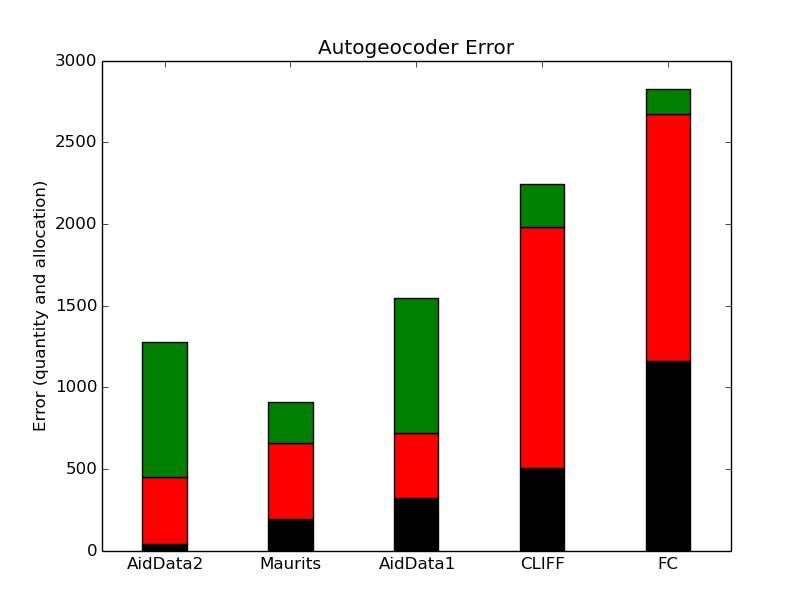
\includegraphics[scale=1.0,width=0.5\textwidth]{compare_plot_20150402.png}
Black bars represent quantity error; red bars additional error introduced by allocating points to ADM1; green bars additional error at ADM2.  The total height of the bar represents total error at ADM2.
\end{wrapfigure}

\vspace{0.25cm}
\textbf{Recommendations}
\begin{enumerate}
\item \textbf{Data Providence and Chains} - We highly recommend that all data used to produce geocoded information is retained, and individual projects are linked to the relevant input information. Some activities are already ongoing to support this - the Data Team is working closely with student geocoder managers to ensure the full chain of the data product is saved. Further, onlining of the disk space funded by VPR will allow for a permanent repository for this data. Once these datasets are available, the REU will work with the Data Team and Geocoders to extract a sample of source documents from projects geocoded during summer 2015. This sample will be used for future tests to allow for absolute comparisons of accuracy, as well as enhance the external validity of these comparisons.
\item \textbf{GeoCoding Funding} - The relatively strong performance of Maurtis' code suggests that gains do remain to be had by continuing to pursue more specialized autogeocoding approaches, if finer scale information is desired.  However, the true rate of gain (in terms of percentage accuracy) is currently unknown due to the limitations of the assessment data.  Until better assessment data can be aquired (ETA summer 2015), it is recommended that we do not continue to fund external GeoCoding efforts, and maintain only a minor in-house focus to prevent a loss of institutional knowledge.  After the summer 2015 information is acquired it will become more feasible to re-engage, as we will have a more representative dataset to provide to partners.
\end{enumerate}

\end{document}
